\documentclass[preview]{standalone}

\usepackage{tikz}

\begin{document}

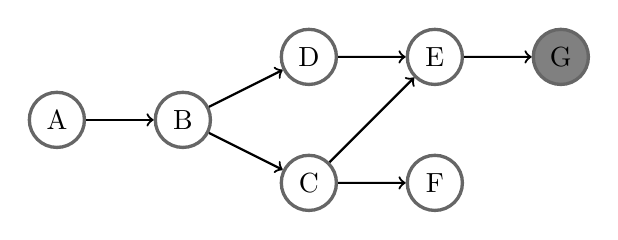
\begin{tikzpicture}
  [scale=.8,auto=left,every node/.style={circle, draw=black!60, very thick, minimum size=7mm}]
  \node (A) at (0,0) {A};
  \node (B) at (2,0) {B};
  \node (C) at (4,-1) {C};
  \node (D) at (4, 1) {D};
  \node (E) at (6,1) {E};
  \node (F) at (6,-1) {F};
  \node (G) [fill=black!50] at (8,1) {G};

  \foreach \from / \to in {A/B, B/C, B/D, D/E, E/G, C/F, C/E}
    \draw[thick, ->] (\from) -- (\to);

\end{tikzpicture}
\end{document}
